\documentclass[11pt, a4paper]{article}
\usepackage[main=galician, spanish]{babel}
\usepackage{fontspec}
\usepackage{libertinus}%%automatically loads aunicode-math package
%%\renewcommand{\familydefault}{\sfdefault}
\usepackage{float}
\usepackage{parskip}
\usepackage[version=4]{mhchem}
\usepackage[figuresleft]{rotating}
\usepackage{graphicx}
\usepackage{amsmath}
\usepackage{slashed}
%\usepackage{amsfonts}
%\numberwithin{equation}{section}%%numbering eqs by section
\usepackage{fancyhdr} 
\usepackage[dvipsnames, table]{xcolor}
\usepackage{wrapfig}
\usepackage[labelfont=bf, skip=4pt, figureposition=bottom, font=normalsize]{caption}
\usepackage{siunitx}
\usepackage{adjustbox}
\usepackage{booktabs} 
\usepackage{multirow}
\usepackage[a4paper,left=2cm,right=2cm,top=2.5cm,bottom=2.5cm]{geometry}
\usepackage{csquotes}
\usepackage{enumitem}
\usepackage{subcaption}
\usepackage{listings}
\usepackage{abstract}
\usepackage{hyperref} 
%%adapted to galician (GZ)
\renewcommand{\tableautorefname}{Cadro}
\usepackage{lipsum}

%% ENUMITEM settings
%\setlist{itemsep=4pt}
\setlist[enumerate,1]{
  label={\bfseries \arabic*.},
}

%% SIUNITX
\sisetup{output-decimal-marker = {,}}
\sisetup{exponent-product= \cdot}
\sisetup{separate-uncertainty=false}
\sisetup{table-parse-only=true}
\sisetup{inter-unit-product = \ensuremath { { } \cdot { } } }
\sisetup{detect-all}
\sisetup{group-digits=integer}
\sisetup{print-unity-mantissa=false}
\sisetup{list-final-separator = { e }}
\sisetup{range-phrase = -}
\sisetup{range-units = single}
\sisetup{list-units = single}
\sisetup{propagate-math-font = true}
\sisetup{text-series-to-math = true}
\sisetup{list-final-separator = { e }}
\sisetup{list-pair-separator = { e }}
\DeclareSIUnit{\espesor}{\milli\g\per\cm\squared}
\DeclareSIUnit{\aten}{\cm\squared\per\milli\g}
\DeclareSIUnit\clight{\text{\ensuremath{c}}}
\DeclareSIUnit\year{a}
\DeclareSIUnit{\barn}{b}
\DeclareSIUnit{\bar}{bar}
\DeclareSIUnit{\neutrons}{\text{neutróns}}
\DeclareSIUnit{\deuterons}{\text{deuteróns}}
\DeclareSIUnit{\counts}{\text{contas}}

%%OTHER COMMANDS
%% for isotopes
\newcommand{\iso}[2]{\ce{^{#1}#2}}
%for vectors
\newcommand{\vect}[1]{\boldsymbol{#1}}
%for ann
\newcommand{\ann}{a_{nn}}
% figure sizes
\newcommand*{\fw}{0.6}
%%for lstlisting package
\definecolor{backcolour}{rgb}{0.95,0.95,0.92}
\lstset{
%backgroundcolor=\color{backcolour},
basicstyle=\small\ttfamily,
language=C++,
keepspaces=false,
keywordstyle=\bfseries\color{Purple},
morekeywords={TSpectrum, TH1, TH1I, TH1D,
Double_t, Int_t, TGraph, TGraphErrors, TMinuit, TF1, TSpline3, G4NistManager,
QGSP_BIC_HP,
SimGeometry, ROOT, Math, XYZPoint, XYZVector, SRIM},
stringstyle=\color{Orange},
identifierstyle=\color{ForestGreen},
breaklines=false,
captionpos=b,
belowskip=-0.85 \baselineskip,
%columns=flexible,
}

\title{\textbf{Guión das prácticas no IGFAE}}
\author{%Miguel Lozano González\\
\small{Prácticas optativas de Grao $\cdot$ Curso 24-25}\\
\small{Universidade de Santiago de Compostela}}
\date{\empty}%\date{\today}

\pagestyle{fancy}
\fancyhf{}
%\fancyhead[R]{\thepage}
\fancyhead[R]{\textsc{guion prácticas igfae}}
\fancyfoot[C]{\thepage}
\renewcommand{\headrulewidth}{0.75pt}
%\renewcommand{\footrulewidth}{0.75pt}
\setlength{\headheight}{14.5pt}

\hypersetup{
	colorlinks=true,
    linkcolor=blue,
    filecolor=magenta,      
    urlcolor=cyan,
}

%% BIBLIOGRAPHY
% \usepackage[
% backend=biber,
% style=numeric,
% sorting=none
% ]{biblatex}
% \addbibresource{./biblio.bib}

%% DOCUMENT

\begin{document}
\begin{minipage}{0.48\linewidth}
    \maketitle
\end{minipage}\hfill
\begin{minipage}{0.48\linewidth}
    \tableofcontents
\end{minipage}

\noindent\rule{\textwidth}{1pt}
% {\renewcommand{\abstractname}{}
% \renewcommand{\absnamepos}{empty}
% \begin{abstract}
% \noindent Memoria das prácticas externas do Mestrado en Física realizadas no Grupo de Física Corpuscular e Aplicacións (FICA), adscrito ao IGFAE (\url{https://igfae.usc.es/igfae/}), baixo a supervisión de Juan Lois Fuentes (\url{juan.lois.fuentes@usc.es}), sendo titora académica Beatriz Fernández Domínguez (\url{beatriz.fernandez.dominguez@usc.es}).
% \end{abstract}
% }
\section{Presentación}
\subsection{Obxectivos}
O obxectivo destas prácticas vai ser de introducir técnicas de \textit{machine learning} na análise de datos do detector \textit{ACtive TARget and Time Projection Chamber} (ACTAR TPC). Máis concretamente, centrarémonos en identificar as partiículas de alta enerxía que superan dous muros de silicio. Trátase dunha técnica novel que nunca se implementou neste tipo de dispositivos, polo que non está garantido que funcione... Pero merece a pena probar e pode ofrecer unha formación moi interesante. 

Abarcaremos varias áreas:
\begin{itemize}
    \item \textbf{Programación}: Afondaremos na programación con \verb|python|, utilizando módulos de \textit{ML} como \verb|tensorflow| ou \texttt{scikit-learn}. Melloraremos os coñecementos de \verb|pandas| e \verb|matplotlib|, así como unha introdución aos \textbf{histogramas} con \verb|hist|.
    
    \item \textbf{Detectores}: ACTAR TPC é un detector gasoso moi recente que abre todo unha nova ventá de posibilidades no eido das reaccións nucleares. Introduciremos os conceptos básicos dun detector gasoso e complementarémolos cos de detectores de silicio, esenciais neste experimento.
    
    \item \textbf{Teoría}: Expoñeremos as leis básicas da cinemática que rixen calquera reacción entre partículas e introduciremos os fundamentos da interacción radiación-materia, básicos neste experimento.
\end{itemize}

Comezaremos estudando os fundamentos teóricos e implmentándoos manualmente para asegurar que se entenden ben. A segunda parte abarcará a parte computacional en si mesma, tentando chegar ao obxectivo final de identificar as partículas.

\subsection{Motivación}
Neste ano levarase a cabo un experimento para estudar reaccións de transferencia co \iso{11}{Li}, de xeito que se poda facer un estudo pormenorizado da súa estrutura nuclear. Estudos coma este son moi importantes, posto que o \textit{modelo de capas nuclear} (moi parecido ao seu análogo atómico) sábese que falla a medida que nos afastamos da estabilidade e pasamos a outros máis exóticos ($N / Z \gg 1$), e faise necesario postular modelos teóricos máis amplos, válidos de forma xenérica.

As reaccións que imos estudar son:
\begin{itemize}
    \item $\iso{11}{Li} + \iso{}{d} \rightarrow \iso{}{p} + \iso{12}{Li}$

    É unha reacción de engádega dun neutrón.
    
    \item $\iso{11}{Li} + \iso{}{d} \rightarrow \iso{}{d} + \iso{11}{Li}$

    É a difusión elástica (E$_{x} = 0$) ou inelástica (E$_x > 0$).
    
    \item $\iso{11}{Li} + \iso{}{d} \rightarrow \iso{}{t} + \iso{10}{Li}$

    Aquí, ao contrario, eliminamos un neutrón.
\end{itemize}

Todo isto é posíbel grazas á seguinte configuración do detector:
\begin{itemize}
    \item \textbf{Gas}: O gas que encherá ACTAR TPC será unha mestura de \ce{D_2} e \ce{CF_4} (\qty{90}{\percent} e \qty{10}{\percent}, respectivamente) a unha presión de \qty{900}{\milli\bar}. Será o \ce{D_2} o que provea os $\iso{}{d}$ da reacción.
    \item \textbf{Feixe}: O \iso{11}{Li} terá unha enerxía de \qty{7.5}{A\MeV} (é dicir, \qty{82.5}{\MeV}), e será producido no acelerador ISAC de TRIUMF, en Canadá.
\end{itemize}

\section{Principios físicos}
\subsection{Un detector gasoso}
ACTAR TPC segue os principios de funcionamento dunha \textit{time projection chamber}: as partículas ao pasaren polo gas ionizan os átomos, liberando electróns que \textbf{derivan} baixo aplicación dun campo eléctrico. Esta carga é recollida nun sensor amplamente fragmentado (), permitindo \textit{seguir} as partículas no seu traspaso dentro do medio en 2D.

Pero é máis: pódese engadir a terceira coordenada coñecendo o tempo que lle leva aos electróns chegar ao \textit{pad plane}, pois a \textbf{velocidade de deriva} é constante. Deste xeito, o seguimento das partículas faise en \textbf{3D}.

Finalmente, o principio de \textit{active target} engade a vantaxe de ser o gas o propio albo da reacción: este actúa como medio de reacción e de detección. O seguinte esquema ilustra este modo de funcionamento.
\begin{figure}[!ht]
    \begin{minipage}[b]{.45\textwidth}
        \centering
        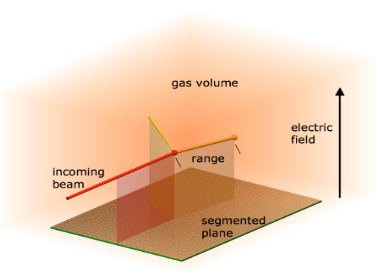
\includegraphics[width=1\textwidth]{figures/tpc.png}
        \caption{Esquema de funcionamento dunha TPC.}
        \label{fig:tpc}
    \end{minipage}
    \hfill
    \begin{minipage}[b]{.45\textwidth}
        \centering
        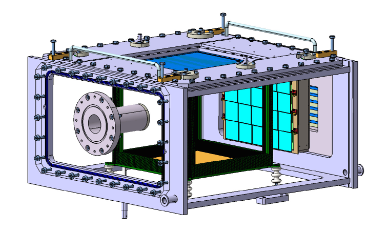
\includegraphics[width=1\textwidth]{figures/actar.png}
        \caption{Deseño do detector ACTAR TPC. A rexión de detección é a parte negra interna.}
        \label{fig:actar}
    \end{minipage}
\end{figure}

Os datos que vas analizar proveñen dunha simulación na cal se implementaron os seguintes parámetros:
\begin{itemize}
    \item O tamaño da zona de detección (\autoref{fig:actar}) é de \qtyproduct[product-units=power]{256 x 256 x 255}{\mm}.
    \item O criterio de dimensións é que o beam vai no eixo X, e a dimensión vertical é Z.
    \item Os detectores auxiliares poden poñerse arredor desta zona nos diferentes lados. Nós usaremos algo parecido ao da figura, cos detectores de Si (como os \textcolor{blue}{azuis}) cara adiante.
    \item Teremos dous muros de silicio, un tras do outro. O primeiro está a \qty{10}{\cm} do \textit{pad plane} e o segundo está separado do primeiro \qty{3}{\cm}. Cada muro constitúese de 12 unidades de tamaño \qtyproduct[product-units=power]{80 x 50 x 1.5}{\mm}.
\end{itemize}

A disposición xeométrica é a que se amosa a continuación.
\begin{figure}[!htb]
    \centering
    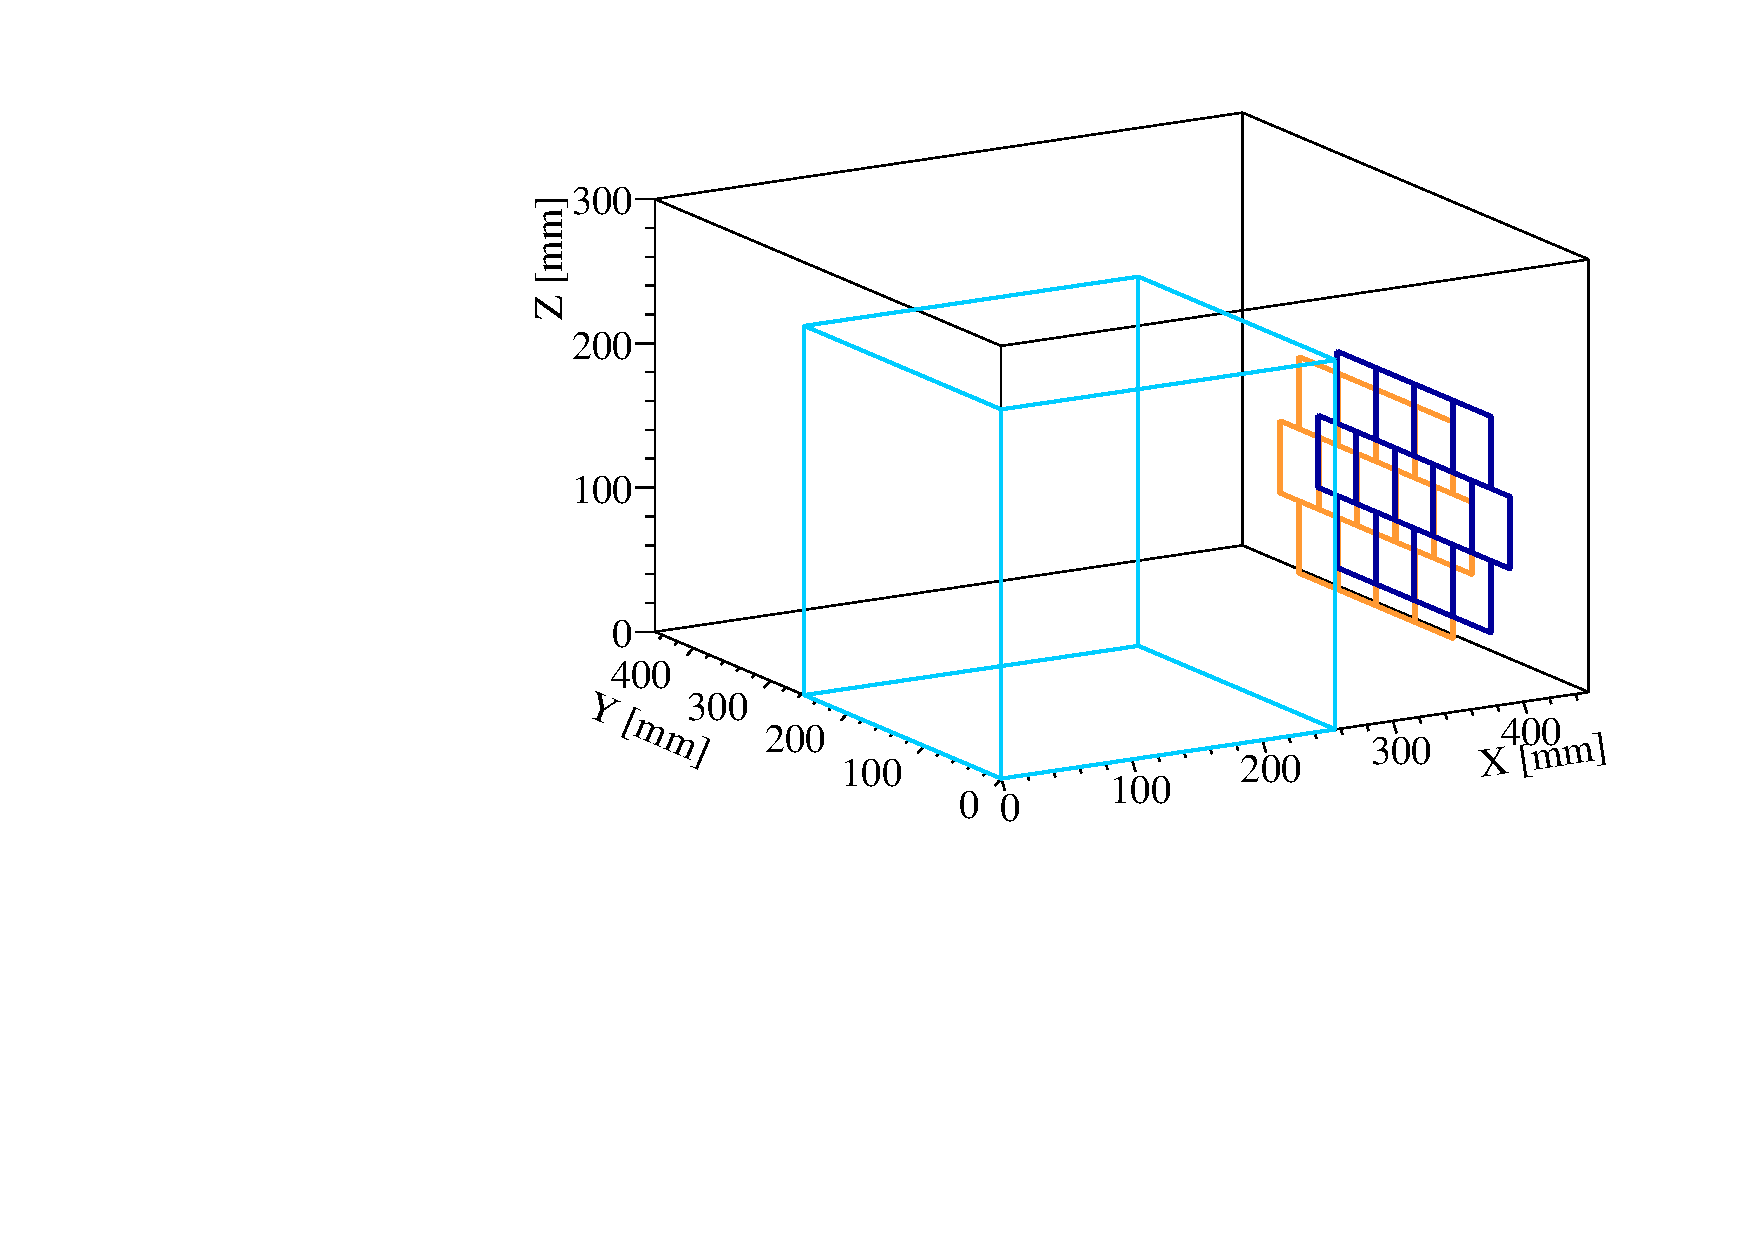
\includegraphics[width=0.7\linewidth]{figures/geo.pdf}
    \caption{O código de cores é o seguinte: \textcolor{Cyan}{ACTAR TPC en azul}, en \textcolor{Blue}{escuro a primeira capa de silicios} e en \textcolor{orange}{laranxa o segundo}.}
\end{figure}

\subsection{Perdas de enerxía na materia}\label{sec:de}
As partículas ao propagarse a través do gas interaccionarán co campo de Coulomb dos átomos deste, perdendo enerxía e liberando electróns. Esta perda de enerxía en cada interacción é moi pequena, pero como é moi elevado o número de colisións no gas (é, polo tanto, un proceso estocástico), chega a ser moi importante. Nunha aproximación continua, está dada pola \textbf{ecuación de Bethe-Bloch}:
\begin{equation*}\label{eq:stopping}
    - \frac{dE}{dx} \cong \frac{4 \pi e^4}{m_e} \left(\rho \frac{N_A}{M}\right)\frac{z^2 Z}{v^2} \ln{\frac{2m_e v^2}{I}}
\end{equation*}
Depende esencialmente da partícula a considerar ($Z$ e $A$) e do gas (a través de $\rho$). É interesante definir:
\begin{itemize}
    \item Rango ($R$): É o camiño percorrido por unha partícula ata que \textit{case} se detén. É función da enerxía inicial e do material a atravesar. Existe unha \textbf{relación unívoca} $E \Longleftrightarrow R$ que imos utilizar para estimar a perda da enerxía en función da distancia percorrida pola partícula.
    \item \textit{Straggling}: Como a perda de enerxía é un \textbf{proceso estatístico}, dúas partículas coa mesma enerxía inicial non van depositar a mesma $\Delta E$. O \textit{straggling} mide, dalgunha forma, a $\sigma$ desta distribución.
\end{itemize}
Esta información está tabulada nun programa que se coñece como \textit{\textbf{SRIM}} e que foi empregado para obter os datos que se analizarán. Non obstante, vas familiarizarte con el para entender ben os conceptos da interación radiación-materia explicados máis arriba.

% Unha pequena apreciación: SRIM vainos dar o \textit{straggling} en posición, mais nós deberémolo converter a en enerxía. Aquí o algoritmo que imos usar:
% \begin{enumerate}
%     \item Calculamos $R_{ini}$ coa enerxía inicial, xunto co seu \textit{straggling}.
%     \item Sabendo que a partícula percorre unha distancia $d$ o rango nese punto será $R_{L} = R_{Ini} - d$. Avaliamos o \textit{stragg.} para este valor.
%     \item O \textit{straggling} na distancia estará \textbf{correlacionado con ambos}, e sabendo que $u^2(R_{Ini}) = u^2(R_{Left}) + u^2(d)$, despexamos $u(d)$.
%     \item Aleatorizamos o valor de $d$ cunha gaussiana centrada no seu valor e de $\sigma = u(d)$. Recalculamos o valor de $R_{Left} \longrightarrow R_{Left}^{\prime}$ coa nova $d \longrightarrow d\prime$.
%     \item Con este novo rango calculamos a enerxía final, efectivamente implementando o \textit{straggling}!
% \end{enumerate}

\subsection{Resolución en enerxía}\label{sec:res}
Complementariamente acostuman situarse detectores de Si que nos van permitir medir a enerxía das partículas á súa saída do \textit{pad plane} (seguindo os mesmos principios que na anterior Sección). Un parámetro importante destes é a \textbf{resolución en enerxía}, definida como a capacidade para \textit{resolver} enerxías depositadas distintas: $R = \textrm{FWHM} / E$.

Para o noso experimento, esta resolución está tabulada en \qty{50}{\keV} a \qty{5.5}{\MeV} e podemos extrapolala ao resto de enerxías coa función:
\begin{equation*}
    R = \frac{2.35 \sigma}{E} = \frac{K}{\sqrt{E}} \quad \implies \quad \sigma = \frac{K}{2.35}\sqrt{E} = \frac{\qty{0.0213}{\MeV}}{2.35} \sqrt{E}
\end{equation*}
Isto vai significar que a perda de enerxía $\Delta E$ que calcules nos Si deberala aleatorizar cunha gaussiana de $\sigma$ obtida coa anterior fórmula.

\subsection{Cinemática}
Todo proceso de interacción entre partículas podes escribirse en termos de variables cinemáticas (enerxías e ángulos) usando as \textbf{leis de conservación} de enerxía e de momento. Esta pode ser descrita no sistema LAB ou no CM (mediante unha transformación Lorentz a un sistema con 3-momento nulo en ambas canles de entrada e saída) do seguinte xeito:

\begin{equation*}
    \begin{gathered}
        \text{No LAB:  }p_1=\left(E_1, \vect{p_1}\right); \; p_2=\left(m_2, \vect{0}\right); \; p_3=\left(E_3, \vect{p_3}\right); \; p_4=\left(E_4, \vect{p_4}\right) \\
        \text{No CM:  }p'_1=\left(E'_1, \vect{p'_1}\right); \;  p'_2=\left(E'_2, -\vect{p'_1}\right); \; p'_3=\left(E'_3, \vect{p'_3}\right); \; p'_4=\left(E'_4, -\vect{p'_3}\right)
    \end{gathered}
\end{equation*}

É estándar asumir unha partícula \textit{target} (a 2) en repouso. O que vamos necesitar para a simulación é:
\begin{itemize}
    \item Partiremos da enerxía cinética $T_1$ do feixe (1) no LAB.
    \item Calculares a transformación Lorentz da canle de entrada ao CM.
    \item Repartiremos a $E_{CM}$ (enerxía total no centro de masas) entre as partículas de saída cun $\theta_{CM}$ e $\phi_{CM}$ aleatorios.
    \item Finalmente, recuperaremos as enerxías de saída de ambas partículas no LAB coa transformación inversa.
    \item Tamén necesitaremos os ángulos no laboratorio, $\theta_{Lab}$ e $\phi_{Lab} = \phi_{CM}$.
\end{itemize}

Algunhas fórmulas que che poden ser interesantes para unha transformación Lorentz en X (o feixe móvese nesa dirección; é un convenio):
\begin{gather*}
    E^{\prime} = \gamma \left(E - \beta p_x\right), \qquad p^{\prime}_{x} = \gamma \left(p_x - \beta E\right)\\
    E = \gamma \left(E^{\prime} + \beta p_{x}^{\prime}\right), \qquad p_x = \gamma \left(p^{\prime}_x + \beta E^{\prime}\right)
\end{gather*}
Onde as variables primadas indican que son no CM. Cando transformes ao final do CM ao LAB terás en conta $\theta_{CM}$: $p_{4,x}^{\prime} = |\vect{p^{\prime}_4}| \cdot\cos(\theta_{CM})$. O ángulo $\phi_{CM}$ non aparece de momento posto que é transversal á transformación.

\section{Para comezar}
\subsection{Introdución a ROOT}
O primeiro de todo é aprender a programar en C++ con \href{https://root.cern.ch/}{ROOT}. No \href{https://github.com/Practicas24/Practicas_24}{repositorio de Github}, dentro da carpeta \textit{Macros}, tes algúns exemplos de como traballar con el. Comeza polo básico e despois vas ver como podes crear histogramas, gráficos e números aleatorios: o básico que necesitamos para estar prácticas.

Velaquí algunha información básica que necesitas para comezar:
\begin{itemize}
    \item ROOT é un código desenvolto polo CERN que permite executar código de C++ sen compilar, mediante o que se coñece como \textbf{macros}:
          \begin{lstlisting}
        $ root -l NomeDoMacro.cxx
    \end{lstlisting}

          Vai executar a función chamada \textit{NomeDoMacro} dentro dese ficheiro. Polo tanto, debes nomear o ficheiro igual que a función principal que conteña dentro. Isto non impide que definas outras funcións dentro do mesmo.
    \item Debes saír sempre da sesión unha vez o programa termina, escribindo
          \lstinline|.q|
    \item ROOT provee de numerosas \textbf{clases} que realizan múltiples funcións: \lstinline|TH1D| (histogramas), \lstinline|TGraph| (gráficos), ... Sempre podes consular a documentación na web cando non saibas como se constrúe ou que funcións ten unha clase. Escribe no teu buscador favorito: \textit{NomeDaClase root cern} e deberías ter a documentación no primeiro resultado.
\end{itemize}

\subsection{Github}
Git é unha ferramenta de control de versións que che permitirá manter un historial do teu código, podendo volver atrás cando sexa necesario. Github é unha web para almacenar repositorios Git. Vamos utilizala para poder revisar o código a distancia.

Para iso, o primeiro é ter unha conta en \url{www.github.com}. Tras unha configuración inicial un pouco tediosa, o plan de traballo é o seguinte, que se debe executar cando fagas cambios importantes ou cando remates a túa sesión de traballo:
\begin{enumerate}
    \item \lstinline|git add .| vai engadir todos os cambios dende o anterior \textit{commit}
    \item \lstinline|git commit| abrirá un editor de texto no que crear unha mensaxe para informar dos cambios. Péchase con \lstinline|Ctrl+S, Ctrl+X|
    \item \lstinline|git push| envía os cambios á nube
\end{enumerate}

\section{Programa}
Desenvolveremos a simulación de forma modular, separando as distintas partes en diferentes macros e xuntando todo ao final.

A proposta é a seguinte:
\begin{itemize}
    \item \textbf{Primeira semana}: Configuración do entorno e familiarización con ROOT. Macros para constuír gráficos e samplear en histogramas.
    \item \textbf{Segunda semana}: Resolución da cinemática e implementación da xeometría.
    \item \textbf{Terceira semana}: Introdución das perdas de enerxía e das distintas resolucións.
    \item \textbf{Cuarta semana}: Estudo sistemático da resolución en $\theta_{Lab}$ para distintas configuracións da xeometría, gases, etc.
    \item \textbf{Quinta semana}: Posibilidade de engardir máis cousas á simulación (en función da evolución) ou comezo da memoria.
\end{itemize}

\subsection{Primeira semana}
Os obxectivos son os seguintes:

\subsubsection*{Cinemática}
Resolverás as ecuacións de cinemática para obter as enerxías cinéticas e ángulos no LAB das dúas partículas finais, aínda que presentando máis atención á pesada. Faino de forma xeral, tal e como está escrito na Sección correspondente. O criterio de números é o seguinte: $1 + 2 \longrightarrow 3 + 4$.

Na simulación, as variables que teremos que introducir nas fórmulas serán as masas, a enerxía do feixe e o ángulo $\theta_{CM}$ (que será aleatorio, como veremos).

\subsubsection*{Macros iniciais}
Quero que fagas dous macros onde me representes as seguintes cousas, usando a axuda do repositorio de Github:
\begin{enumerate}
    \item Representacións \textbf{cinemáticas}: Creas un \lstinline|TCanvas| con 3 \textit{pads} e representas a cinemática para estas tres reaccións distintas: $\iso{11}{Li}(d, p)\iso{12}{Li}$, $\iso{11}{Li}(d, d)\iso{11}{Li}$ e $\iso{11}{Li}(d, t)\iso{10}{Li}$. Usa a mesma enerxía do feixe para todas de \qty{7.5}{A\MeV}.

          A clase que vai facer iso é \lstinline|ActPhysics::Kinematics|. O criterio que debes usar para chamar ao constructor é o seguinte: \lstinline|("feixe", "target", "lixeira", "pesada", Tbeam)|, que configura a equivalencia coas fórmulas matemáticas do seguinte xeito: $$1 (\text{feixe}) + 2 (\text{target}) \longrightarrow 3 (\text{lixeira}) + 4 (\text{pesada})$$
          Ademais, \lstinline|GetKinematicLine3()| darache a representación $T_3$ vs $\theta_{Lab, 3}$ (polo tanto, da partícula marcada como \textit{lixeira}) e \lstinline|GetKinematicLine4()| o mesmo pero da 4, a pesada. Representa ambas no mesmo \textit{pad}.

          Vas ver como as formas son moi diferentes, o que forza a deseñar experimentos moi distintos en función da reacción a medir (ou un que sexa capaz de medir todas as canles de reacción).

    \item \textbf{Sampleado} de variables: Para a simulación vamos necesitar samplear variables gaussianas e uniformes. Crea un macro con 3 histogramas (que vas representar en 3 \textit{pads}) distintos nos que samplees as seguintes distribucións (podes xogar cos parámetros como queiras);
          \begin{itemize}
              \item Gaussiana: \lstinline|gRandom->Gaus(mean, sigma)|
              \item Uniforme: \lstinline|gRandom->Uniform(x0, x1)|
              \item O ángulo polar $\theta$ é especial se queres obter unha \href{https://mathworld.wolfram.com/SpherePointPicking.html}{distribución uniforme}:
                    $$\theta = \arccos\left(\texttt{gRandom->Uniform(-1, 1)}\right)$$
          \end{itemize}
          Nota que este ángulo vai estar en radiáns. Para converter a graos, debes multiplicar polo factor de conversión correspondente. Se non o queres escribir, podes usar \lstinline|TMath::RadToDeg()| (a inversa é \lstinline|TMath::DegToRad()|) de ROOT.
\end{enumerate}

\subsection{Segunda semana}
\subsubsection*{Representación gráfica da perda de enerxía}
Na carpeta \lstinline|SRIM| do repositorio tes táboas de perda de enerxía calculadas con SRIM. Se abres unha vas ver toda a información que conteñen:
\begin{itemize}
    \item Información do material no que se calculou a perda.
    \item O mesmo sobre a partícula que o vai atraversar.
    \item Múltiples columnas coa $E$, o rango, o \textit{straggling} en rango e o $dE/dx$.
\end{itemize}
Para ler e traballar con esta clase vas utilizar a clase \lstinline|ActPhysics::SRIM|, tal e como tes no macro de exemplo (\lstinline|Macros/srim.cxx|). As funcións básicas que necesitas son estas:
\begin{itemize}
    \item \lstinline|EvalDirect()|: obtén o rango para unha enerxía dada.
    \item \lstinline|EvalInverse()|: enerxía para un rango dado.
    \item \lstinline|Slow()|: para unha enerxía inicial, calcula a enerxía final tras atravesar un espesor de material a especificar. Tamén lle podes dar un ángulo, de xeito que a lonxitude efectiva é: $l_{\text{eff} = l / \cos{\theta}}$. O ángulo debe especificarse en radiáns.
    \item \lstinline|EvalInitialEnergy()|: cos mesmos argumentos que a anterior función, fai o proceso inverso: calcula a enerxía inicial dada unha enerxía final, lonxitude e opcionalmente ángulo.
\end{itemize}
En todas as funcións o primeiro argumento é unha \textit{string} que especifica a táboa a usar, anteriormente lida con \lstinline|ReadTable()|.

O que quero que fagas é que plotees a perda de enerxía no gas en función da distancia. Para iso, escolle unha táboa (por exemplo, \iso{11}{Li} no gas) e asume unha enerxía inicial. Calcula o rango da partícula a esa enerxía.

Despois, discretiza esa distancia nun intervalo suficientemente pequeno e nun bucle \textit{for}, utilizando a función \lstinline|Slow|, calculas a perda de enerxía (como a diferenza entre as iteracións). Representa iso en dous  \lstinline|TGraph|s: un de perda de enerxía vs distancia e outro de perda de enerxía vs enerxía.

Vas ver unha característica moi importante no gráfico: a medida que a partícula se para, a perda de enerxía aumenta: é o que se coñece como \textbf{pico de Bragg}. Estas dúas características (o perfil de perda de carga e o pico de Bragg) permiten identificar as partículas nun detector, xa que son unha pegada única de cada partícula!

\subsubsection*{Valicación da cinemática}
Crea un macro sinxelo no que definas as funcións necesarias para calcular a cinemática. Mira o exemplo \lstinline|Macros/funcs.cxx| para ver como podes devolver varios parámetros nunha función e escolle a forma que máis che guste.

Unha vez fagas isto, no propio macro vas validar que todo funcione ben. Escolle a reacción $\iso{11}{Li}(d, t)\iso{10}{Li}$ a \qty{7.5}{A\MeV} e segue os seguintes pasos:
\begin{itemize}
    \item Crea un \lstinline|TGraph|.
    \item Nun bucle for, vas percorrer unha variable $\theta_{CM} \in [0, 180]\unit{\degree}$.
    \item Utiliza as túas funcións para calcular $T_{4}, \theta_{Lab, 4}$.
    \item Enche o gráfico.
\end{itemize}
Representa isto nun \lstinline|TCanvas| e \textbf{superimpón} a cinemática de \lstinline|ActPhysis::Kinematics::GetKinematicLine4()|, tal e como aprendiches a facer na anterior semana. Debería quedar exactamente igual!

\subsection{Terceira semana}
\subsubsection*{Comezo da simulación}
Unha vez aprendido o básico, vamos comezar co macro de simulación. O primeiro é adaptar o que acabas de aprender de sampleado:
\begin{enumerate}
    \item Define o tamaño de ACTAR ao comezo do macro en \unit{\mm}. Tes os tamaños ao principio deste guión. En cada iteración, nunha variable tipo \lstinline|XYZPoint| garda:
          \begin{itemize}
              \item X: uniforme na dirección do feixe.
              \item Y e Z: gaussianas de media o centro do detector e de $\sigma$ uns \qty{5}{\mm}. Os feixes de partículas creados nos aceleradores non son perfectos e teñen unha determinada anchura espacial. De momento, asumimos un caso sinxelo de dispersión gaussiana dun feixe ben centrado no detector.
          \end{itemize}
          Podes crear puntos e vectores no espazo coas clases definidas en \lstinline|#include "Math/Point3D.h| e \\ \lstinline|#include "Math/Vector3D.h"|. Podes acceder a elas como \lstinline|ROOT::Math::XYZPoint| ou \\ \lstinline|ROOT::Math::XYZVector|.

          Valida que todo vai ben: crea dous histogramas 2D para representar isto:
          \begin{itemize}
              \item Un onde representes Y vs X.
              \item Outro no que representes Z vs Y.
          \end{itemize}
          \item  Fai o mesmo para os ángulos no CM: samplea e crea histogramas para representalos.

          \item   O seguinte será usar a clase de \textbf{cinemática} que creaches para obter as variables da partícula pesada. Cos ángulos sampleados e coa enerxía do feixe, calcula $T_4$ e $\theta_{4}$.
          
          Representa nun histograma 2D que todo vai ben: nun plot de enerxía fronte a ángulo deberías reproducir a cinemática teórica.

          \item  A continuación, vamos implementar a xeometría do silicio que vai medir esta partícula pesada. Na variable de tipo \lstinline|ActSim::Geometry| está implementada a xeometría do detector, tal e como se ve na seguinte \autoref{fig:geo}. 

          \begin{figure}[!htb]
              \centering
              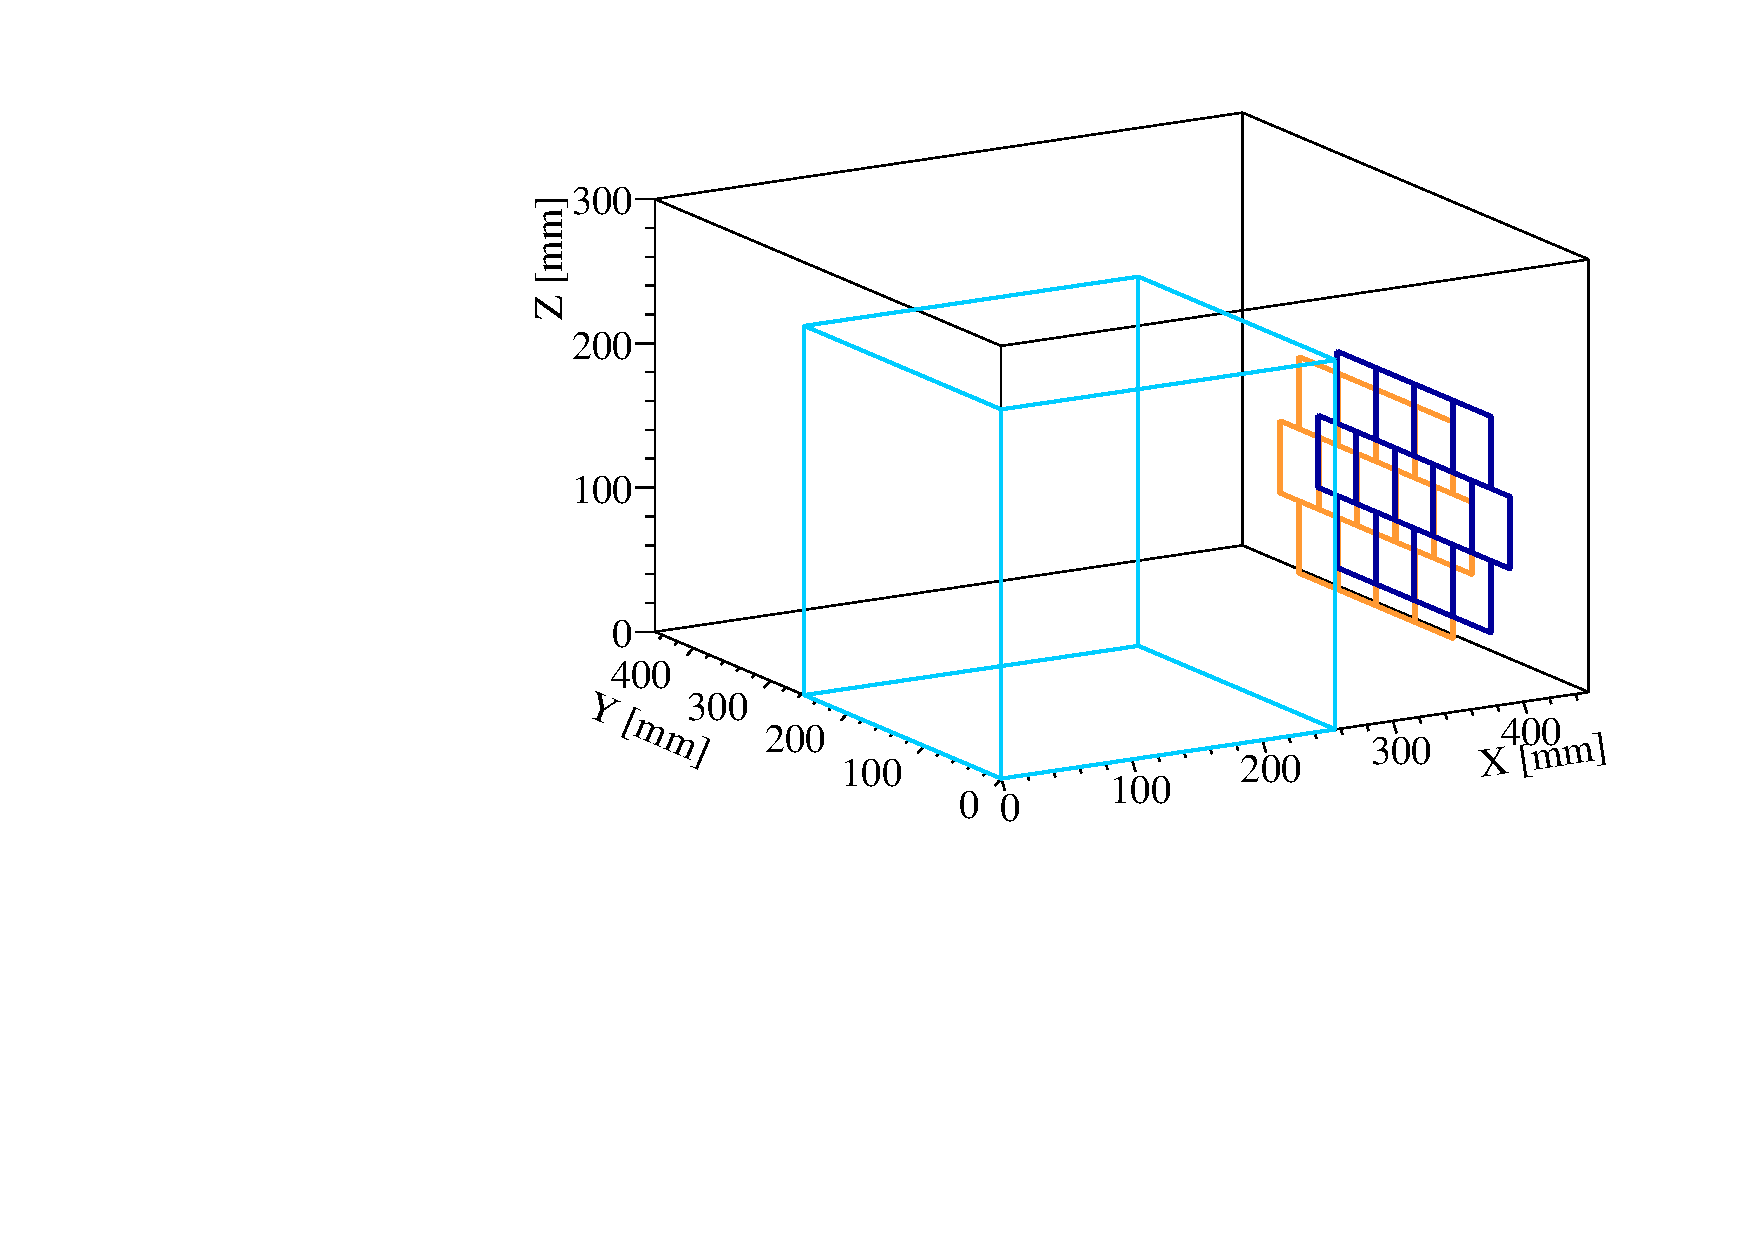
\includegraphics[width=0.5\linewidth]{figures/geo.pdf}
              \caption{Esquema da xeometría: en azul, a TPC; en vermello, o silicio.}
              \label{fig:geo}
          \end{figure}

          Esta clase contén todos os tamaños necesarios para simular a xeometría, cos seguintes valores
          \begin{itemize}
              \item Os tamaños da TPC normal
              \item Os do Si, de \qtyproduct[product-units=power]{80 x 50 x 1.5}{\mm}
              \item Unha distancia de \qty{10.4}{\cm}
          \end{itemize}

          A función que imos utilizar é \lstinline|PropagateTrackToSiliconArray()|. Os argumentos que necesitas son uns cantos:
          \begin{itemize}
              \item O \textbf{vértice}, tal e como sampleaches.
              \item A \textbf{dirección} da partícula. Debes definila do seguinte xeito:
                    \begin{lstlisting}
        ROOT::Math::XYZVector direction {TMath::Cos(theta4), TMath::Sin(theta4) * TMath::Sin(phi4),
                                         TMath::Sin(theta4) * TMath::Cos(phi4)};

    \end{lstlisting}
              \item O índice do muro de silicions, xa que pode haber varios. Como só hai un, pasa un 0.
              \item Os seguintes argumentos van \textbf{devolver} o resultado da operación, e deberás pasar as variables obrigatoriamente:
                    \begin{itemize}
                        \item Un \lstinline|bool| co lado. Ignoraremos isto de momento.
                        \item A distancia dende o vertice ao punto de impacto, en \textbf{\unit{\cm}}. Debes convertela a \unit{\mm}. É a variable máis importante.
                        \item O tipo de silicio. Só hai un, así que ignorarémolo.
                        \item O índice do silicio. Moi importante tamén: se a partícula non chega ao silicon, vale -1.
                        \item Un \lstinline|XYZPoint| co punto de impacto. Ignorarémolo.
                    \end{itemize}
          \end{itemize}

          Deste xeito, só os eventos que cheguen xeometricamente ao silicio terán un valor de \lstinline|silIndex != -1|, e o máis importante, terás a distancia que teñen que viaxar para chegar alí.

          A primeira vez que necesites usar a xeometría debes creala. Hai un macro na carpeta \textit{Geo/Build.cxx} que tes que executar só unha vez. Isto vai crear un ficheiro \textit{.root} cos parámetros necesarios que despois lerás como: \lstinline|geo.ReadGeometry("./Geo/", "simple");|

          \item Finalmente, para os eventos que chegan, representa a enerxía $T_4$ na entrada do silicio: é dicir, usa a variable de tipo \lstinline|SRIM| para reducir a perda de enerxía no gas. Represéntaa respecto do ángulo nun histograma 2D.

          Para iso, terás que usar a táboa de enerxía correspondente. O que che recomendo é ler a táboa do \iso{12}{Li} e que a chames \textit{heavy}, para non evitar malentendidos despois, posto que usaremos as táboas de varias partículas.
          \item Remata calculando a $\Delta E$ da partícula nos silicios. Deberás ter en conta o ángulo coa normal ao chamar a función \lstinline|SRIM::Slow|. Para iso, computa o $\theta$ entre o vector dirección anteriormente calculado e a normal \lstinline|ROOT::Math::XYZVector normal {1, 0, 0}|.

          Deberás usar unha táboa de enerxía distinta! A correspondente da partícula no silicio. Recoméndoche que a chames \textit{heavySil} para diferenciala da \textit{heavy} no gas.
\end{enumerate} 
\subsubsection*{Implementación dos defectos experimentais}
Froito das incertezas estatísticas do proceso de perda de enerxía e das limitacións de contrución e electrónicas do detector, as liñas cinemáticas non son unha \textit{liña} senón unha distribución de valores.

O obxetivo da simulación é ver como, en función da configuración do detector, se dispersas estas liñas e como iso nos afecta na extracción de resultados. Dúas son as que imos implementar:
\begin{enumerate}
    \item \textbf{\textit{Straggling} en enerxía:} Segue o exposto na \autoref{sec:de} para implementalo. Deberás crear unha función que substitúa á \lstinline|SRIM::Slow|, de forma que pasándolle o obxecto \lstinline|SRIM|, unha enerxía inicial $T_{ini}$ e unha distacia $d$ devolva o valor reducido e aleatorizado convenientemente.
    \item \textbf{Resolución dos Si:} como viches na \autoref{sec:res}, os silicios teñen unha incerteza na determinación da enerxía. Dispersa o valor de $\Delta E$ obtido neles creando unha función que aplique a fórmula. 
\end{enumerate}
\end{document}
